\chapter{Introduction}

\section{Goals}

The following thesis aims to provide insight into threat assessment and mitigation, regarding ambient intelligence systems.
In order to achieve this, several main discussion directions are proposed - architectural modifications, threat analysis, correction
methods, detection schemes and feedback polynomial study.

Firstly, the proposed architecture for the system is network-based, being more versatile and providing an increased abstraction level
to the final system. The network, or intelligent grid, is comprised of intelligent agents, each managing an individual resource, leading
to more efficient workloads at the cost of dependability. Given that each resource being being used separately, with minimum oversight,
there is no innate guarantee that a given resource is not malicious.

Because of the aforementioned security risk, a thorough threat assessment is done in order to ascertain system reliability. This can
be achieved through an analysis of error occurrence, resulting in a threat model that will help understand and prevent future vulnerabilities.
At the same time, it will also allow for quick response to any identified malicious resource used by an intelligent agent.

On top of threat detection, a correction step is included, were an error to be introduced into the system. Such errors can occur due to
the transceiver nature of the intelligent grid nodes, with the messages sent between agents being corrupted by external factors. Because of
this, from an architectural point of view, the transmission layer should handle authentication and eventual error correction steps.

While threat assessment and error correction deal with the consequences of a potential attack, detection schemes manage threat identification.
The proposed method of achieving such a scheme is to identify previously unknown attack patterns, associate it to a specific signature and
compile all signatures into a dictionary, for future lookup, thus being able to check for the given signature in the future. In order to
construct the detection scheme, a feedback polynomial has to be identified, based on the available metrics.

Finally, the most important aspect of this thesis is promoting the aforementioned ideas concerning the reliability of the intelligent grid,
with regard to security and fault tolerance. The end goal is to begin a discussion about the design of a fully secured system, starting
from the presented paradigms.

\section{Design}

Due to the presented intelligent grid being emulated on current hardware, it is required that the overall system is reliable, in terms of
resource allocation and access, and inter-agent communication protocols. As such, the final design is meant for reliability, meaning that
it takes into account deviations that appear between system and specification \cite{36, 113}.

Another aspect promoting a reliable system is that of cost, more specifically, the proportional relationship between cost and security -
the investment has do double in order for the vulnerability count to halve. At the same time, the security errors and their effects can
generate costs measured in billions of dollars \cite{113, 114}. For this reason, the final design is done in accordance to the following
principles:

\begin{figure}[H]
	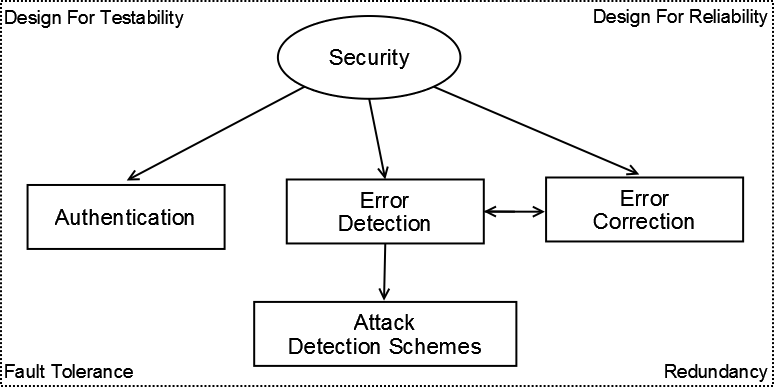
\includegraphics[width=0.9\textwidth, height=0.65\textwidth]{Pic1}
	\caption{Security mechanisms and designing principles \label{fig:designPrinciples}}
\end{figure}

As shown in \cref{fig:designPrinciples}, the goals set for this thesis cover several security directions, and are doubled by design principles
coupled with their respective mechanisms. The design aims to measure the improvements caused by different techniques, such that the final
system is designed to be tested based on relative risk measures.

